\documentclass[12pt]{article}
\usepackage{../preamble3}
%\pagenumbering{gobble}
\title{MathCounts Chapter Invitational February 2021 \\ Sprint Round}
\author{Patrick \& James Toche}
\date{Revised:~\today}

\begin{document}
\maketitle
\begin{minipage}{\textwidth}
\begin{abstract}\setlength{\parindent}{0pt}%
Notes on Sprint Round of MathCounts Invitational Competition, February 2021. 
Questions are from MathCounts Foundation (\url{https://www.mathcounts.org/}). Copyright restrictions may apply. Written for personal use. 
Please report typos and errors over at \url{https://github.com/ptoche/Math/tree/master/mathcounts}. 
\end{abstract}
\end{minipage}

\thispagestyle{empty}
\clearpage
\addtocounter{page}{-1}

\section*{Sprint Round}


%%%%%%%%%%%%%%%%%%%%%%%%%%%%%%%%%%%%%%%%%%%%%%%%%%%%%%%%%%%%%%%%%%%%%%%%
\subsection*{1.}
What is the arithmetic mean of the terms in the arithmetic sequence $12$, $18$, $24$, $30$, $36$?

\nopagebreak

\fbox{\phantom{ANSWER}}

\begin{answer}
You could calculate it ($(12+18+24+30+36)/5=24$), but you can get the result without calculations by noting that the mean of an arithmetic sequence is its median, that is if $a$ denotes the increment, we have:
\begin{center}
\begin{tabular}{Q{2cm}Q{2cm}Q{2cm}Q{2cm}Q{2cm}}
   12, &   18, & 24, & 30,   & 36 \\
24-2a, & 24-a, & 24, & 24+a, & 24+2a
\end{tabular}
\end{center}
When you calculate the sum, the $-2a$ term is canceled by $+2a$ and $-a$ is canceled by $+a$, leaving $(5 \times 24)/5=24$.
\begin{empheq}[box={\mathbox[colback=white]}]{equation*}
    24
\end{empheq}
\end{answer}
%%%%%%%%%%%%%%%%%%%%%%%%%%%%%%%%%%%%%%%%%%%%%%%%%%%%%%%%%%%%%%%%%%%%%%%%


%%%%%%%%%%%%%%%%%%%%%%%%%%%%%%%%%%%%%%%%%%%%%%%%%%%%%%%%%%%%%%%%%%%%%%%%
\subsection*{2.}
If Skylar colors $\dfrac{1}{2}$ of $\dfrac{2}{3}$ of the squares in this figure, how many squares does he color?

\begin{minipage}[b]{\linewidth}
  \centering
  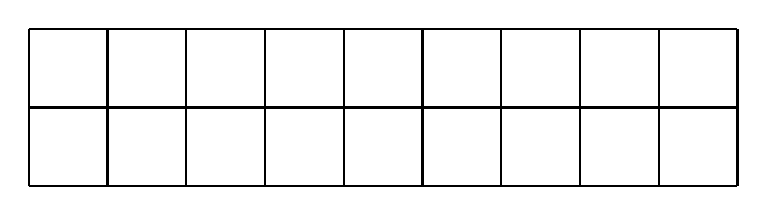
\begin{tikzpicture}
  \foreach \x in {1,...,10}{
    \draw[thick] (\x,0) -- (\x,2) {};
    }
  \foreach \y in {0,...,2}{
    \draw[thick] (1,\y) -- (10,\y) {};
    }
  \end{tikzpicture}
\end{minipage}

\nopagebreak

\fbox{\phantom{ANSWER}}~squares

\begin{answer}
There are $9$ columns and $2$ rows. Two-thirds of $9$ columns gives $6$ columns, half of that gives $3$ columns, so $3 \times 2 = 6$.
\begin{empheq}[box={\mathbox[colback=white]}]{equation*}
    6 ~\text{squares}
\end{empheq}
\end{answer}
%%%%%%%%%%%%%%%%%%%%%%%%%%%%%%%%%%%%%%%%%%%%%%%%%%%%%%%%%%%%%%%%%%%%%%%%


%%%%%%%%%%%%%%%%%%%%%%%%%%%%%%%%%%%%%%%%%%%%%%%%%%%%%%%%%%%%%%%%%%%%%%%%
\subsection*{3.}
What is the median of the first seven prime numbers?

\nopagebreak

\fbox{\phantom{ANSWER}}

\begin{answer}
The first seven prime numbers are:
\begin{align*}
2, 3, 5, 7, 11, 13, 17
\end{align*}
so the median is the number in the middle, $7$. 
\begin{empheq}[box={\mathbox[colback=white]}]{equation*}
    7
\end{empheq}
\end{answer}
%%%%%%%%%%%%%%%%%%%%%%%%%%%%%%%%%%%%%%%%%%%%%%%%%%%%%%%%%%%%%%%%%%%%%%%%


%%%%%%%%%%%%%%%%%%%%%%%%%%%%%%%%%%%%%%%%%%%%%%%%%%%%%%%%%%%%%%%%%%%%%%%%
\subsection*{4.}
What is the absolute difference between five less than a number $n$ and seven more than $n$?

\nopagebreak

\fbox{\phantom{ANSWER}}

\begin{answer}
The verbal statement may be expressed as
\begin{align*}
|(n-5) - (n+7)| = |-12| = 12
\end{align*}
\begin{empheq}[box={\mathbox[colback=white]}]{equation*}
    12
\end{empheq}
\end{answer}
%%%%%%%%%%%%%%%%%%%%%%%%%%%%%%%%%%%%%%%%%%%%%%%%%%%%%%%%%%%%%%%%%%%%%%%%


%%%%%%%%%%%%%%%%%%%%%%%%%%%%%%%%%%%%%%%%%%%%%%%%%%%%%%%%%%%%%%%%%%%%%%%%
\subsection*{5.}
What is the distance between points $A$ and $B$ on the coordinate grid shown? 

\begin{minipage}[b]{\linewidth}
  \centering
  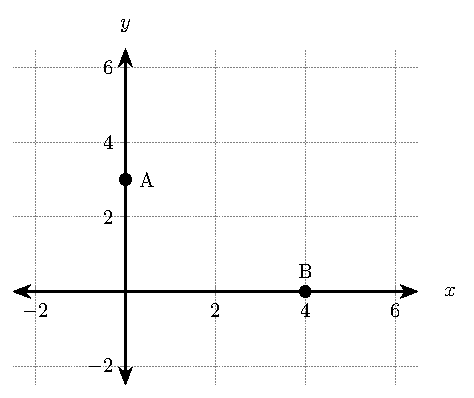
\includegraphics[height=7cm]{sprint-05-figure}
\end{minipage}

\nopagebreak

\fbox{\phantom{ANSWER}}~units

\begin{answer}
The distance between $A$ and $B$ is the hypotenuse of the triangle with side lengths $3$ and $4$. Therefore
\begin{align*}
\sqrt{3^2 + 4^2} = 5
\end{align*}
This of course is the best-known of the Pythagorean triangles $(3,4,5)$. 
\begin{empheq}[box={\mathbox[colback=white]}]{equation*}
    5 ~\text{units}
\end{empheq}
\end{answer}
%%%%%%%%%%%%%%%%%%%%%%%%%%%%%%%%%%%%%%%%%%%%%%%%%%%%%%%%%%%%%%%%%%%%%%%%


%%%%%%%%%%%%%%%%%%%%%%%%%%%%%%%%%%%%%%%%%%%%%%%%%%%%%%%%%%%%%%%%%%%%%%%%
\subsection*{6.}
Regular hexagon $ABCDEF$, shown here, has area $5$ units$^2$. What is the area of trapezoid $BCDE$? Express your answer as a decimal to the nearest tenth. 

\begin{minipage}[b]{\linewidth}
  \centering
  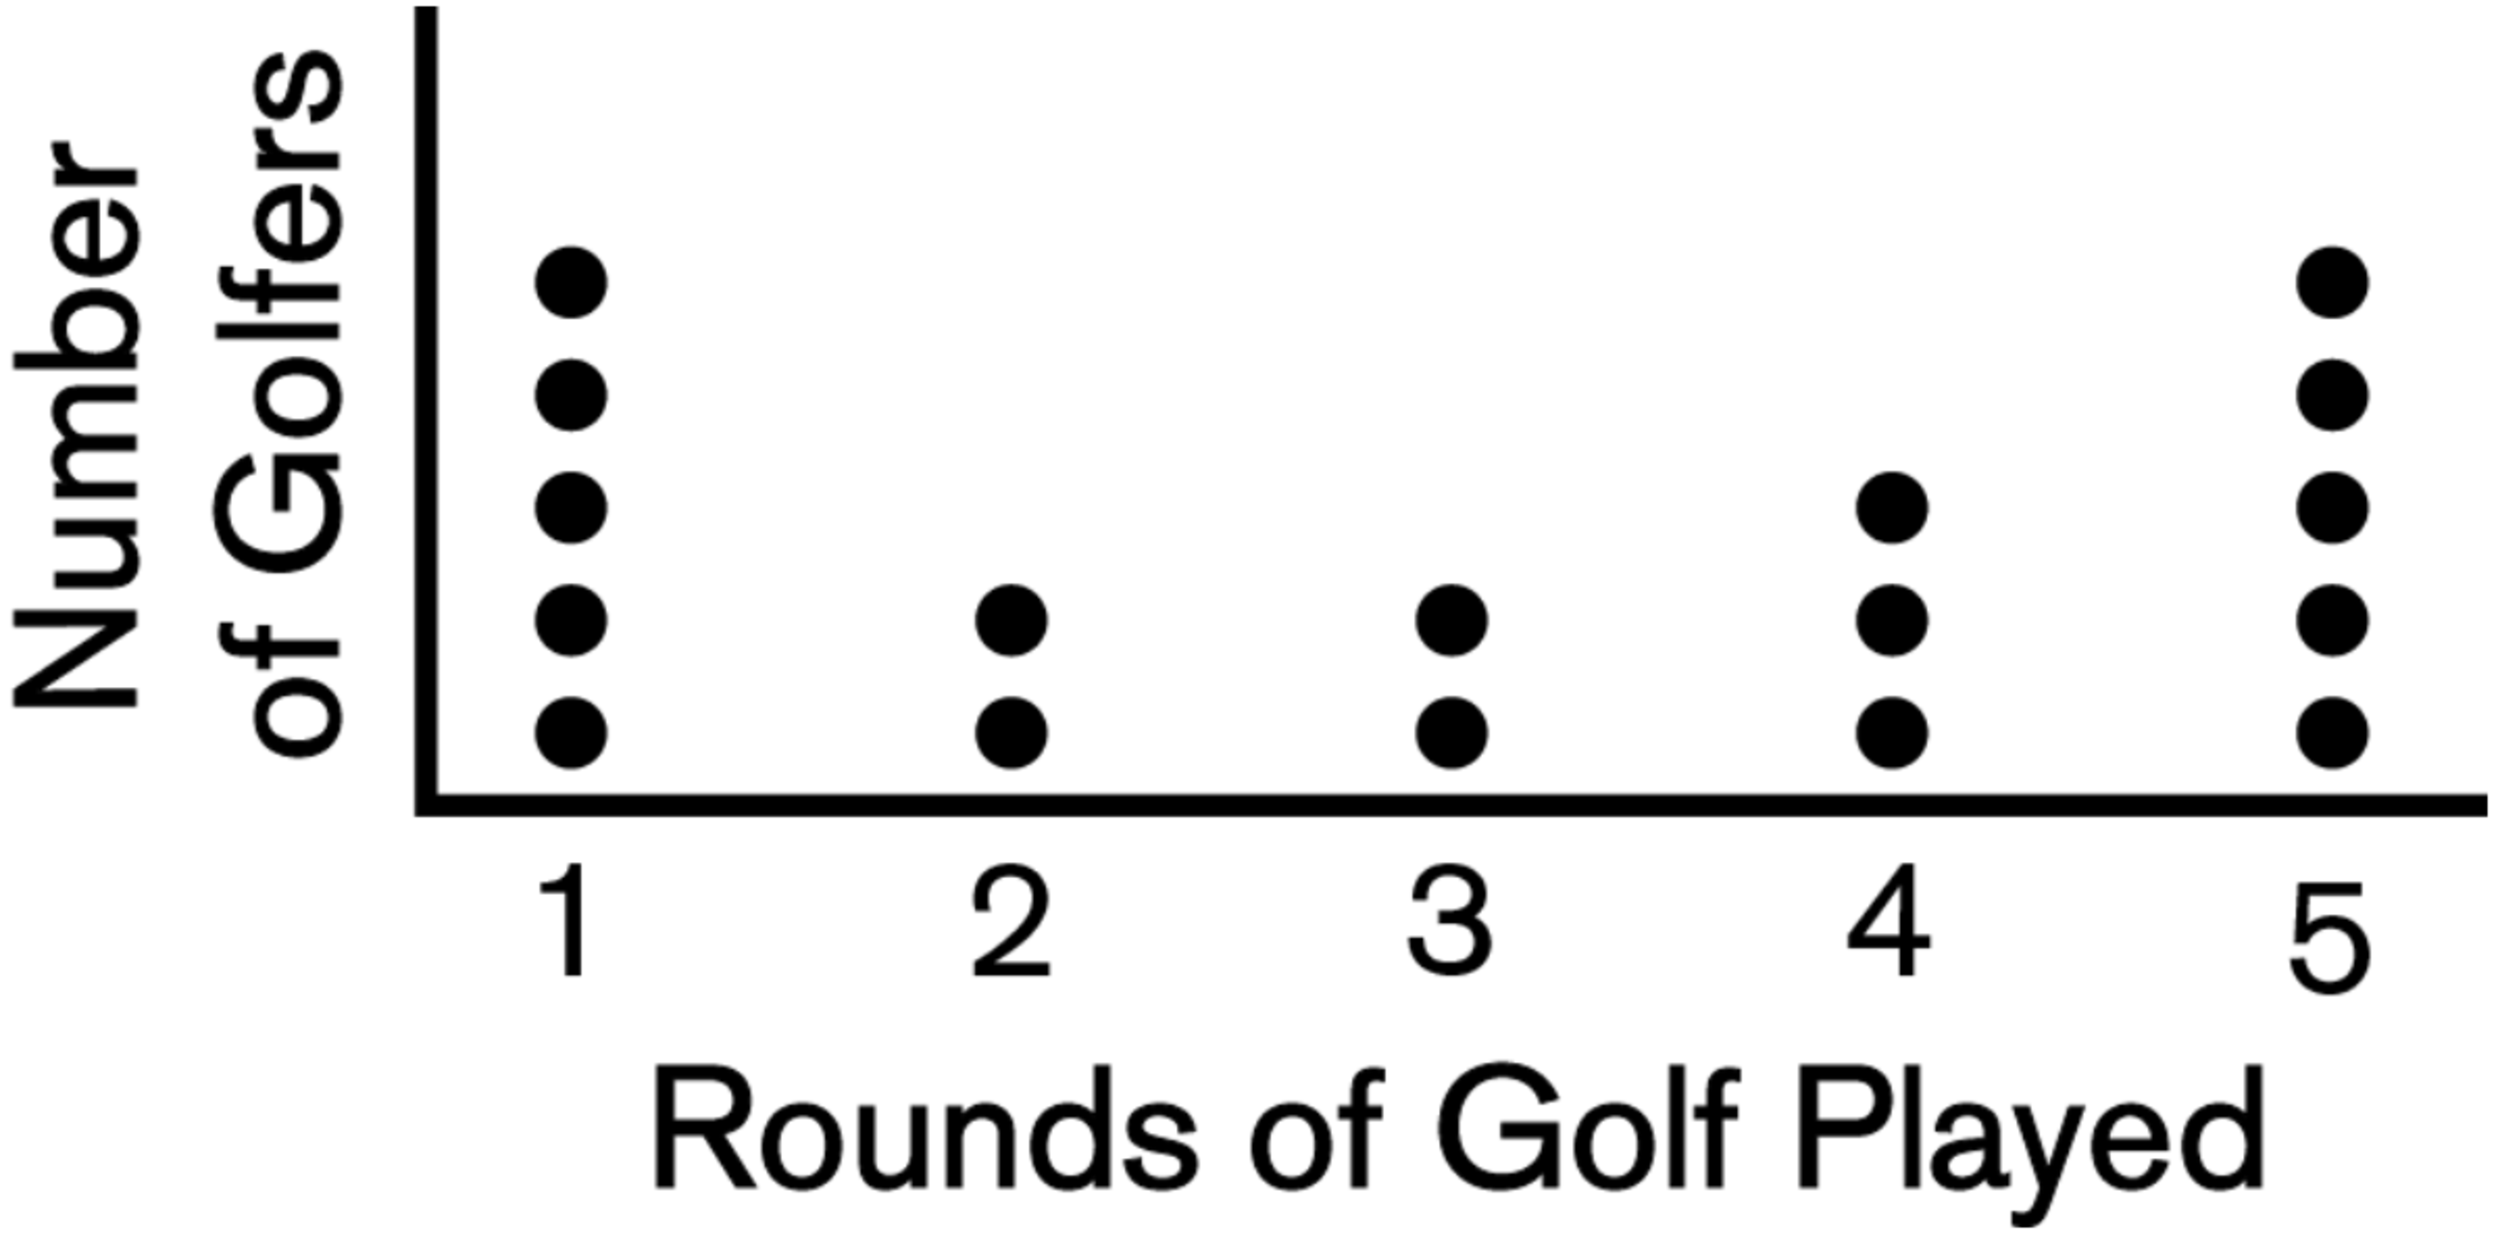
\includegraphics[height=5cm]{sprint-06-figure}
\end{minipage}

\nopagebreak

\fbox{\phantom{ANSWER}}~units$^2$

\begin{answer}
The area of trapezoid $BCDE$ is clearly half of hexagon $ABCDEF$.
\begin{empheq}[box={\mathbox[colback=white]}]{equation*}
    2.5 ~\text{units}^2
\end{empheq}
\end{answer}
%%%%%%%%%%%%%%%%%%%%%%%%%%%%%%%%%%%%%%%%%%%%%%%%%%%%%%%%%%%%%%%%%%%%%%%%


%%%%%%%%%%%%%%%%%%%%%%%%%%%%%%%%%%%%%%%%%%%%%%%%%%%%%%%%%%%%%%%%%%%%%%%%
\subsection*{7.}
What is the value of the expression $\sqrt{9^2-5 \times 4 + 12 \div 4}$

\nopagebreak

\fbox{\phantom{ANSWER}}

\begin{answer}
Respecting the order of operations:
\begin{align*}
\sqrt{9^2-5 \times 4 + 12 \div 4}
  = \sqrt{81-20 + 3}
  = \sqrt{64}
  = 8
\end{align*}
\begin{empheq}[box={\mathbox[colback=white]}]{equation*}
    8
\end{empheq}
\end{answer}
%%%%%%%%%%%%%%%%%%%%%%%%%%%%%%%%%%%%%%%%%%%%%%%%%%%%%%%%%%%%%%%%%%%%%%%%


%%%%%%%%%%%%%%%%%%%%%%%%%%%%%%%%%%%%%%%%%%%%%%%%%%%%%%%%%%%%%%%%%%%%%%%%
\subsection*{8.}
Given that $3a+5=7b-11$ and $a=b$, what is the value of $a$?

\nopagebreak

\fbox{\phantom{ANSWER}}

\begin{answer}
This simple system of two equations in two unknowns may be solved by substitution:
\begin{align*}
3a + 5 & = 7a - 11 \\ 
    4a & = 16 \\
     a & = 4
\end{align*}
\begin{empheq}[box={\mathbox[colback=white]}]{equation*}
    4
\end{empheq}
\end{answer}
%%%%%%%%%%%%%%%%%%%%%%%%%%%%%%%%%%%%%%%%%%%%%%%%%%%%%%%%%%%%%%%%%%%%%%%%


%%%%%%%%%%%%%%%%%%%%%%%%%%%%%%%%%%%%%%%%%%%%%%%%%%%%%%%%%%%%%%%%%%%%%%%%
\subsection*{9.}
An album with twelve songs costs $\$9.99$. If Andy buys each song individually, he pays $\$0.99$ per song. How much money can Andy save by buying the album instead of each individual song?

\nopagebreak

\fbox{\phantom{ANSWER}}

\begin{answer}
Andy can save:
\begin{align*}
12 \times 0.99 - 9.99  
  & = (12 \times 1 - 12 \times 0.01) - (10 - 0.01) \\
  & = 2 - 11 \times 0.01 \\
  & = 2 - 0.1 + 0.01 \\
  & = 1.89
\end{align*}
\begin{empheq}[box={\mathbox[colback=white]}]{equation*}
    \$~ 1.89
\end{empheq}
\end{answer}
%%%%%%%%%%%%%%%%%%%%%%%%%%%%%%%%%%%%%%%%%%%%%%%%%%%%%%%%%%%%%%%%%%%%%%%%


%%%%%%%%%%%%%%%%%%%%%%%%%%%%%%%%%%%%%%%%%%%%%%%%%%%%%%%%%%%%%%%%%%%%%%%%
\subsection*{10.}
What is the integer value of \faPaw ~$\bm{+}$~ \faBirthdayCake ~$\bm{+}$~ \faAutomobile, given these three equations?
\begin{align*}
% The symbols used by MathCounts were:
% \faPaw -> Dog
% \faBirthdayCake -> Ice Cream
% \faAutomobile -> Turtle
\text{\faPaw} ~\bm{+}~ \text{\faPaw} ~\bm{+}~ \text{\faPaw} & \bm{~=~ 90} \\
\text{\faPaw} ~\bm{+}~ \text{\faBirthdayCake} ~\bm{+}~ \text{\faBirthdayCake} & \bm{~=~ 60} \\
\text{\faPaw} ~\bm{+}~ \text{\faPaw} ~\bm{-}~ \text{\faAutomobile} & \bm{~=~ 40}
\end{align*}

\nopagebreak

\fbox{\phantom{ANSWER}}

\begin{answer}
\begin{align*}
 \bm{3}~\text{\faPaw} & \bm{~=~ 90 \quad\Rightarrow\quad \text{\faPaw} = 30} \\
 \bm{2}~\text{\faBirthdayCake} & \bm{~=~ 60 -
\text{\faPaw} \quad\Rightarrow\quad  \text{\faBirthdayCake} = 15} \\
\text{\faAutomobile} & \bm{~=~ 2~\text{\faPaw} -40 = 20} \\
\Rightarrow\quad \text{\faPaw} ~\bm{+}~ \text{\faBirthdayCake} ~\bm{+}~ \text{\faAutomobile} & \bm{~=~ 30 + 15 + 20 = 65} 
\end{align*}
    \begin{empheq}[box={\mathbox[colback=white]}]{equation*}
        65
    \end{empheq}
\end{answer}
%%%%%%%%%%%%%%%%%%%%%%%%%%%%%%%%%%%%%%%%%%%%%%%%%%%%%%%%%%%%%%%%%%%%%%%%


%%%%%%%%%%%%%%%%%%%%%%%%%%%%%%%%%%%%%%%%%%%%%%%%%%%%%%%%%%%%%%%%%%%%%%%%
\subsection*{11.}
At Alicia's new job, she works three days a week for a total of $45$ hours per week. At her old job, she worked $4$ days a week for a total of $40$ hours per week. What is the absolute difference in the average number of hours Alicia worked per workday at her old and new jobs?

\nopagebreak

\fbox{\phantom{ANSWER}}~hours

\begin{answer}
Alicia can save:
\begin{align*}
\left|\frac{45}{3} - \frac{40}{4}\right|
  = |15 - 10|
  = 5
\end{align*}
\begin{empheq}[box={\mathbox[colback=white]}]{equation*}
    5 ~\text{hours}
\end{empheq}
\end{answer}
%%%%%%%%%%%%%%%%%%%%%%%%%%%%%%%%%%%%%%%%%%%%%%%%%%%%%%%%%%%%%%%%%%%%%%%%


%%%%%%%%%%%%%%%%%%%%%%%%%%%%%%%%%%%%%%%%%%%%%%%%%%%%%%%%%%%%%%%%%%%%%%%%
\subsection*{12.}
What is the value of $x$ if $x^x = 256$?

\nopagebreak

\fbox{\phantom{ANSWER}}

\begin{answer}
Since $256$ is a power of $2$, so must be $x$. Candidates are then $2$, $4$, $8$, and so on. Thus,
\begin{align*}
x^x = 256 \Rightarrow 4^4 = 256 
\end{align*}
\begin{empheq}[box={\mathbox[colback=white]}]{equation*}
    4
\end{empheq}
\end{answer}
%%%%%%%%%%%%%%%%%%%%%%%%%%%%%%%%%%%%%%%%%%%%%%%%%%%%%%%%%%%%%%%%%%%%%%%%


%%%%%%%%%%%%%%%%%%%%%%%%%%%%%%%%%%%%%%%%%%%%%%%%%%%%%%%%%%%%%%%%%%%%%%%%
\subsection*{13.}
What is the least positive integer that has five distinct prime factors?

\nopagebreak

\fbox{\phantom{ANSWER}}

\begin{answer}
Multiply the first five prime numbers:
\begin{align*}
2 \times 3 \times 5 \times 7 \times 11 = 3 \times 770 = 2310
\end{align*}
\begin{empheq}[box={\mathbox[colback=white]}]{equation*}
    2310
\end{empheq}
\end{answer}
%%%%%%%%%%%%%%%%%%%%%%%%%%%%%%%%%%%%%%%%%%%%%%%%%%%%%%%%%%%%%%%%%%%%%%%%


%%%%%%%%%%%%%%%%%%%%%%%%%%%%%%%%%%%%%%%%%%%%%%%%%%%%%%%%%%%%%%%%%%%%%%%%
\subsection*{14.}
Jasmine estimates her maximum heart rate, in beats per minute, by subtracting her age from $220$. Jasmine's heart rate during exercise should be between $50\%$ and $85\%$ of her maximum heart rate. If Jasmine is $20$ years old, what is the highest heart rate, in beats per minute, that she should have during exercise? Express your answer to the nearest whole number. 

\nopagebreak

\fbox{\phantom{ANSWER}}~beats per minute

\begin{answer}
The highest rate Jasmine should have, $r_{\text{max}}$, is:
\begin{align*}
r_{\text{max}} 
  = 0.85 \times r
  = 0.85 \times (220 - 20)
  = 170	
\end{align*}
\begin{empheq}[box={\mathbox[colback=white]}]{equation*}
    170 ~\text{beats per minute}
\end{empheq}
\end{answer}
%%%%%%%%%%%%%%%%%%%%%%%%%%%%%%%%%%%%%%%%%%%%%%%%%%%%%%%%%%%%%%%%%%%%%%%%


%%%%%%%%%%%%%%%%%%%%%%%%%%%%%%%%%%%%%%%%%%%%%%%%%%%%%%%%%%%%%%%%%%%%%%%%
\subsection*{15.}
The arithmetic mean of three distinct integers is $11$, and the range of the three integers is $2$. What is the smallest of these integers?

\nopagebreak

\fbox{\phantom{ANSWER}}

\begin{answer}
Since the range is $2$, these are three consecutive integers, with the middle integer being $11$, implying that the smallest of the three is $10$. 
\begin{empheq}[box={\mathbox[colback=white]}]{equation*}
    10
\end{empheq}
\end{answer}
%%%%%%%%%%%%%%%%%%%%%%%%%%%%%%%%%%%%%%%%%%%%%%%%%%%%%%%%%%%%%%%%%%%%%%%%


%%%%%%%%%%%%%%%%%%%%%%%%%%%%%%%%%%%%%%%%%%%%%%%%%%%%%%%%%%%%%%%%%%%%%%%%
\subsection*{16.}
Let $a\&b=ab+b+a-1$. If $a\&7=70$, what is $a\&3$?

\nopagebreak

\fbox{\phantom{ANSWER}}~

\begin{answer}
A simple matter of substituting $7$ for $b$:
\begin{align*}
a\&7 = 70 
\quad\Rightarrow\quad 
7a + 7 + a - 1 = 70 
\quad\Rightarrow\quad 
a = \frac{70-6}{8} = 8
\end{align*}
and then substituting both $8$ for $a$ and $3$ for $b$:
\begin{align*}
a\&3 = 8\&3 = 8 \times 3 + 3 + 8 - 1 = 34
\end{align*}
\begin{empheq}[box={\mathbox[colback=white]}]{equation*}
    34
\end{empheq}
\end{answer}
%%%%%%%%%%%%%%%%%%%%%%%%%%%%%%%%%%%%%%%%%%%%%%%%%%%%%%%%%%%%%%%%%%%%%%%%

\iftoggle{showAnswers}{\newpage}

%%%%%%%%%%%%%%%%%%%%%%%%%%%%%%%%%%%%%%%%%%%%%%%%%%%%%%%%%%%%%%%%%%%%%%%%
\subsection*{17.}
Kody's alarm rings every $11$ minutes, and his dad calls upstairs every $15$ minutes to wake him up. But Kody will only wake up if his alarm rings and his dad calls him at the same time. If his alarm first rings at $7{:}00$am and his dad first calls him at $7{:}05$a.m., at what time will Kody wake up?

\nopagebreak

\fbox{\phantom{ANSWER}}~a.m.

\begin{answer}
\begin{minipage}[b]{\linewidth}
  \centering
  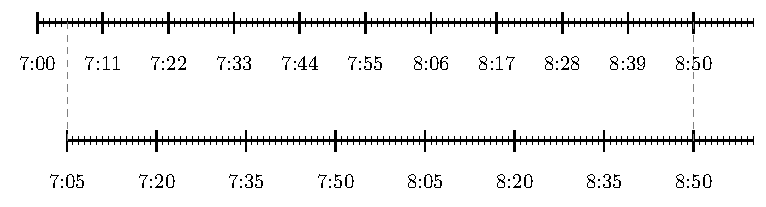
\includegraphics[height=4cm]{sprint-17-figure}
\end{minipage}              
  We are looking for the ``smallest'' pair of integers $(u,v)$ such that:
  \begin{align*}
  7\,\text{hours} + (11u)\,\text{minutes} = 7\,\text{hours} + (5 + 15v)\,\text{minutes}
  \end{align*}
  or equivalently:
  \begin{align*}
  11u = 5(1 + 3v)
  \end{align*}
  It follows that $u$ must be a multiple of $5$, while $1+3v$ must be a multiple of $11$. Since we are looking for ``small'' values of $u$ and $v$, we can start guessing with $u=5,10,15$, etc.. 
  \begin{align*}
  u & = 5 \quad \frac{11 \times 5}{5} = 11 = 1 + 3v  \Rightarrow v = \frac{10}{3} \quad \notin\mathbb{N} \quad\text{\faTimes} \\
  u & = 10 \quad \frac{11 \times 5}{10} = 22 = 1 + 3v \Rightarrow v = \frac{21}{3} = 7 \quad \in\mathbb{N} \quad\text{\faCheck}
  \end{align*}
  Our second attempt yields a solution: $u=10$, $v=7$,
  implying that Kody wakes up at $7\,\text{hours}$ and $110\,\text{minutes}$ or, equivalently $8\,\text{hours}$ and $50\,\text{minutes}$. 
  \begin{empheq}[box={\mathbox[colback=white]}]{equation*}
      8{:}50 ~\text{a.m.}
  \end{empheq}
\end{answer}
%%%%%%%%%%%%%%%%%%%%%%%%%%%%%%%%%%%%%%%%%%%%%%%%%%%%%%%%%%%%%%%%%%%%%%%%

\iftoggle{showAnswers}{\newpage}

%%%%%%%%%%%%%%%%%%%%%%%%%%%%%%%%%%%%%%%%%%%%%%%%%%%%%%%%%%%%%%%%%%%%%%%%
\subsection*{18.}
The largest rectangular region shown is partitioned into three rectangular regions labeled $A$, $B$, and $C$. The lengths, in inches, of rectangles $A$, $B$, and $C$ are $n+3$, $n+5$ and $n-2$, respectively, and all three rectangles have width $n$. If the area of rectangle $B$ is $84$in$^2$, what is the perimeter of the largest rectangle shown?

\begin{center}
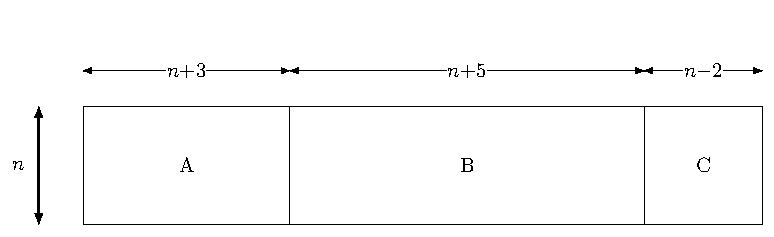
\includegraphics[height=5cm]{sprint-18-figure}
\end{center}

\nopagebreak

\fbox{\phantom{ANSWER}}~inches

\begin{answer}
The area of rectangle $B$ is $n(n+5)$, which yields a quadratic equation in $n$:
\begin{align*}
   n^2 + 5n = 84
\end{align*}
Completing the square:
\begin{align*}
   n^2 + 5n & = 84 \\
   \left(n + \frac{5}{2}\right)^2 - \left(\frac{5}{2}\right)^2 & = 84 \\
   \left(n + \frac{5}{2}\right)^2 - \left(\frac{25+4 \times 84}{2^2}\right) & = 0 \\
   \left(n + \frac{5}{2}\right)^2 - \left(\frac{19}{2}\right)^2 & = 0 
\end{align*}
where the last step follows from $25+4\times84=25+336=361=19^2$.
To complete the square, recall that $a^2-b^2=(a-b)(a+b)$. Thus,
\begin{align*}
   \left(n+\frac{5}{2}-\frac{19}{2}\right)  \left(n+\frac{5}{2}+\frac{19}{2}\right) & = 0 \\
   (n-7)(n+12) & = 0 
\end{align*}
(This solution could have been guessed if we had had good reasons to believe that the solutions were integers)
Since $n$ must be positive, $n=7$. 
The perimeter of the largest rectangle is 
\begin{align*}
2 \times [n + (n+3) + (n+5) + (n-2)] 
  = 2 (4n+6) 
  = 2 (28+6)
  = 68
\end{align*}
\begin{empheq}[box={\mathbox[colback=white]}]{equation*}
    68 ~\text{inches}
\end{empheq}
\end{answer}
%%%%%%%%%%%%%%%%%%%%%%%%%%%%%%%%%%%%%%%%%%%%%%%%%%%%%%%%%%%%%%%%%%%%%%%%

\iftoggle{showAnswers}{\newpage}

%%%%%%%%%%%%%%%%%%%%%%%%%%%%%%%%%%%%%%%%%%%%%%%%%%%%%%%%%%%%%%%%%%%%%%%%
\subsection*{19.}
What is the length of the longest diagonal of the rectangular prism shown, which has length $9$\,cm, width $8$\,cm and height $12$\,cm?

\begin{center}
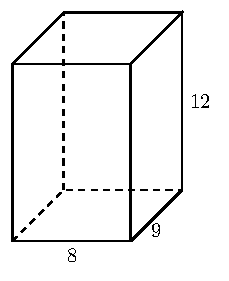
\includegraphics[height=6cm,page=1]{sprint-19-figure}
\end{center}

\nopagebreak

\fbox{\phantom{ANSWER}}~cm

\begin{answer}
The longest diagonal along the surface of the prism is clearly \begin{align*}
\sqrt{9^2+12^2} = \sqrt{81+144} = \sqrt{225} = 15
\end{align*}
But it is readily apparent that the ``inner'' diagonal --- the red line in the figure below --- is longer. The length of the red, dotted diagonal is:
\begin{align*}
\sqrt{9^2+8^2} = \sqrt{81+64} = \sqrt{145} ~~(\approx 12)
\end{align*}
\begin{center}
\includegraphics[height=6cm,page=2]{sprint-19-figure}
\end{center}
Putting it together yields:
\begin{align*}
\sqrt{145+144} = \sqrt{289} = 17
\end{align*}
Quick calculation: If the width/length/height of a rectangular prism are $x$, $y$, $z$, the longest diagonal has length $\sqrt{x^2+y^2+z^2}$.
\begin{empheq}[box={\mathbox[colback=white]}]{equation*}
    17 ~\text{cm}
\end{empheq}
\end{answer}
%%%%%%%%%%%%%%%%%%%%%%%%%%%%%%%%%%%%%%%%%%%%%%%%%%%%%%%%%%%%%%%%%%%%%%%%

\iftoggle{showAnswers}{\newpage}

%%%%%%%%%%%%%%%%%%%%%%%%%%%%%%%%%%%%%%%%%%%%%%%%%%%%%%%%%%%%%%%%%%%%%%%%
\subsection*{20.}
Suppose there is an $80\%$ chance of rain each day. On days that it rains, Kathy has a $45\%$ chance of being late, compared to a $30\%$ chance when it does not rain. On a random day, what is the probability that Kathy will be late?

\nopagebreak

\fbox{\phantom{ANSWER}}~\%

\begin{answer}
On a random day, the probability of being late can be broken down into rainy and dry days (see the probability tree):
\begin{center}
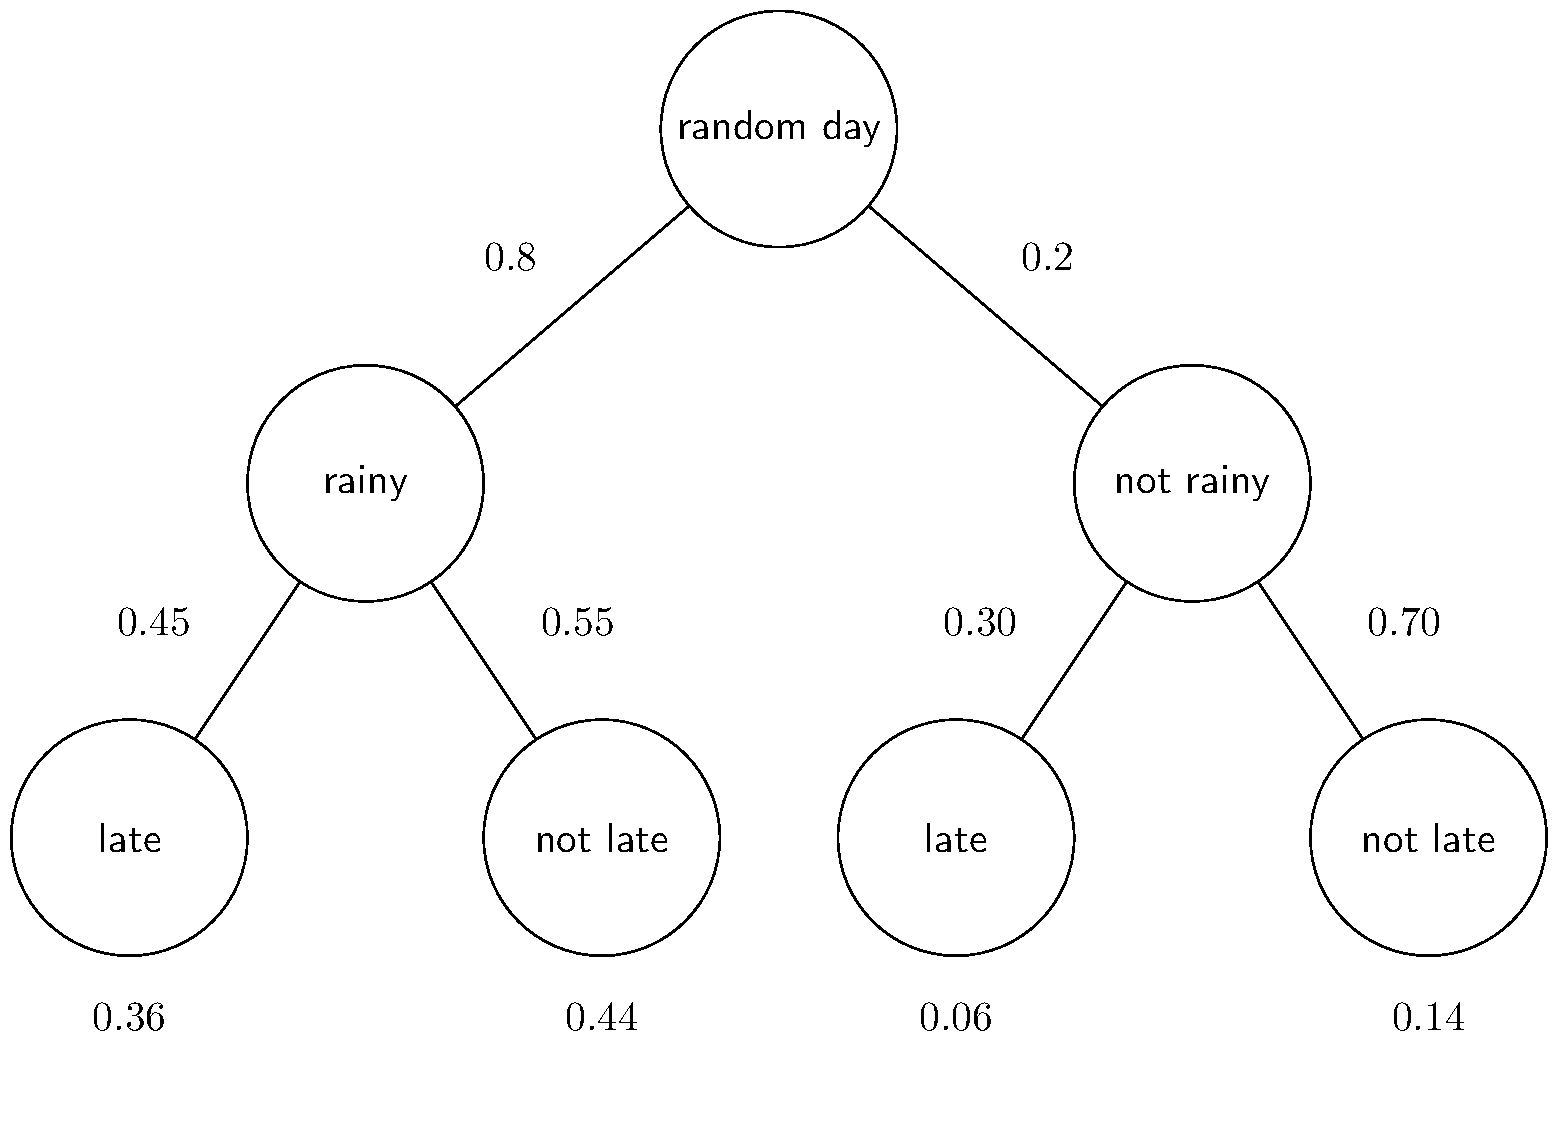
\includegraphics[height=8cm]{sprint-20-figure}
\end{center}
\begin{align*}
\underbrace{0.8 \quad\times\quad 0.45}_{\text{rainy day}} 
\quad + \quad
\underbrace{0.2 \quad\times\quad 0.3}_{\text{dry day}}
  \quad=\quad 0.36 \quad+\quad 0.06
  \quad=\quad 0.42
% 0.8 * 0.45 + (1-0.8) * 0.3
\end{align*}
\begin{empheq}[box={\mathbox[colback=white]}]{equation*}
    42 \%
\end{empheq}
\end{answer}
%%%%%%%%%%%%%%%%%%%%%%%%%%%%%%%%%%%%%%%%%%%%%%%%%%%%%%%%%%%%%%%%%%%%%%%%

\iftoggle{showAnswers}{\newpage}

%%%%%%%%%%%%%%%%%%%%%%%%%%%%%%%%%%%%%%%%%%%%%%%%%%%%%%%%%%%%%%%%%%%%%%%%
\subsection*{21.}
Triangle $ABC$ has sides of length $11$ inches, $15$ inches and $16$ inches. What is the length of the altitude to the side of length $15$ inches? Express your answer in simplest radical form. 

\nopagebreak

\fbox{\phantom{ANSWER}}$\sqrt{\fbox{\phantom{ANSWER}}}$

\begin{answer}
We start by drawing the basic figure:
\begin{center}
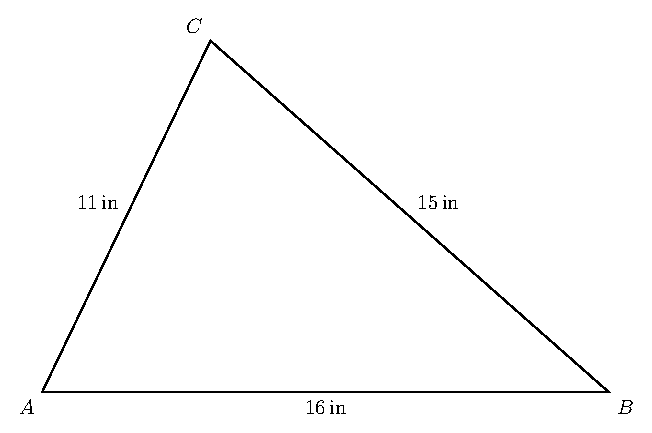
\includegraphics[height=8cm,page=1]{sprint-21-figure}
\end{center}
We add the projection of $A$ onto segment $BC$ and label the unknown lengths $x$ and $y$. 
\begin{center}
\includegraphics[height=8cm,page=2]{sprint-21-figure}
\end{center}
Applying the Pythagoras theorem to triangles $APC$ and $APB$ yields a system of two equations in two unknowns:
\begin{align*}
x^2 + y^2 & = 11^2 \\
x^2 + (15-y)^2 & = 16^2
\end{align*}
While the system appears to be non-linear, it may be simplified. Develop the square in the second equation:
\begin{align*}
x^2 + 15^2 - 30 y + y^2 = 16^2
\end{align*}
Substitute the first equation into the above and rearrange:
\begin{align*}
30 y & = 11^2 - 16^2 + 15^2\\
y & = \frac{90}{30} = 3
\end{align*}
With $y$ we can now find $x$:
\begin{align*}
x^2 & = 11^2 - 3^2 = 112 \\
  x & = \sqrt{112} = 4 \sqrt{7}
\end{align*}
Putting the solution into the figure:
\begin{center}
\includegraphics[height=7cm,page=3]{sprint-21-figure}
\end{center}
\begin{empheq}[box={\mathbox[colback=white]}]{equation*}
    4\sqrt{7}
\end{empheq}
\end{answer}
%%%%%%%%%%%%%%%%%%%%%%%%%%%%%%%%%%%%%%%%%%%%%%%%%%%%%%%%%%%%%%%%%%%%%%%%

\iftoggle{showAnswers}{\newpage}

%%%%%%%%%%%%%%%%%%%%%%%%%%%%%%%%%%%%%%%%%%%%%%%%%%%%%%%%%%%%%%%%%%%%%%%%
\subsection*{22.}
Julie is packing marbles into boxes. She needs to pack away $815$ marbles. She has boxes that can hold $10$, $25$, $50$ or $100$ marbles. If Julie can use at most $5$ boxes of each size and must fill each box she uses, what is the minimum number of boxes she needs to pack all her marbles?

\nopagebreak

\fbox{\phantom{ANSWER}}~boxes

\begin{answer}
Starting with the maximal feasible number of the larger boxes --- $5$ items per box --- and going down from there, we get close but not quite there: 
\begin{align*}
5 \times 100 \quad+\quad 5 \times 50 \quad+\quad 2 \times 25 \quad+\quad 1 \times 10 \quad=\quad 810 \quad<\quad 815
\end{align*}
The total number of boxes must be at least $14$.
If we remove one $25$-box and complement with several $10$-box, we now get to $815$ marbles:
\begin{align*}
5 \times 100 \quad+\quad 5 \times 50 \quad+\quad 1 \times 25 \quad+\quad 4 \times 10 \quad=\quad 815
\end{align*}
for a total number of boxes:
\begin{align*}
5 + 5 + 1 + 4 = 15
\end{align*}
\begin{empheq}[box={\mathbox[colback=white]}]{equation*}
    15 ~\text{boxes}
\end{empheq}
\end{answer}
%%%%%%%%%%%%%%%%%%%%%%%%%%%%%%%%%%%%%%%%%%%%%%%%%%%%%%%%%%%%%%%%%%%%%%%%


%%%%%%%%%%%%%%%%%%%%%%%%%%%%%%%%%%%%%%%%%%%%%%%%%%%%%%%%%%%%%%%%%%%%%%%%
\subsection*{23.}
What positive number $x$ has the property that $\sqrt[6]{x^7}-6\sqrt[3]{x^2}=0$?

\nopagebreak

\fbox{\phantom{ANSWER}}

\begin{answer}
It is easier to manipulate fractional exponents:
\begin{align*}
\sqrt[6]{x^7} & \,=\, 6\sqrt[3]{x^2} \\
x^{\frac{7}{6}} & \,=\, 6x^{\frac{2}{3}} \\
x^{\frac{7}{6}-\frac{2}{3}} & \,=\, 6 \\
x^{\frac{3}{6}} & \,=\, 6 \\
x^{\frac{1}{2}} & \,=\, 6 \\
x & \,=\, 6^2 \\
x & \,=\, 36
\end{align*}
\begin{empheq}[box={\mathbox[colback=white]}]{equation*}
    36
\end{empheq}
\end{answer}
%%%%%%%%%%%%%%%%%%%%%%%%%%%%%%%%%%%%%%%%%%%%%%%%%%%%%%%%%%%%%%%%%%%%%%%%


%%%%%%%%%%%%%%%%%%%%%%%%%%%%%%%%%%%%%%%%%%%%%%%%%%%%%%%%%%%%%%%%%%%%%%%%
\subsection*{24.}
What fraction is equivalent to $0.7\overline{12}$? Express your answer as a common fraction. 

\nopagebreak

\begin{minipage}[b]{\linewidth}
\fbox{\phantom{ANSWER}}\\
\mbox{---------------}\\
\fbox{\phantom{ANSWER}}
\end{minipage}


\begin{answer}
\begin{align*}
   x & \,=\, 0.7\overline{12} \\
100x & \,=\, 71.\overline{21} \\
 99x & \,=\, 71.2\overline{12} - 0.7\overline{12} \\
     & \,=\, 71.2 - 0.7 \,=\, 70.5\\
   x & \,=\, \frac{705}{990} \,=\, \frac{47}{66}
\end{align*}
We can easily see that $705$ and $990$ are both divisible by three. In other cases reducing the fraction may be a little more challenging. 
\begin{empheq}[box={\mathbox[colback=white]}]{equation*}
    \frac{47}{66}
\end{empheq}
\end{answer}
%%%%%%%%%%%%%%%%%%%%%%%%%%%%%%%%%%%%%%%%%%%%%%%%%%%%%%%%%%%%%%%%%%%%%%%%

\iftoggle{showAnswers}{\newpage}

%%%%%%%%%%%%%%%%%%%%%%%%%%%%%%%%%%%%%%%%%%%%%%%%%%%%%%%%%%%%%%%%%%%%%%%%
\subsection*{25.}
In the figure, two circles of radius $1$ inch are internally tangent to a circle of radius $5$ inches so that the centers of all tree circles are collinear. The shaded fourth circle is tangent to each of the other three circles as shown. What is the radius of the shaded circle? Express your answer as a common fraction. 

\begin{center}
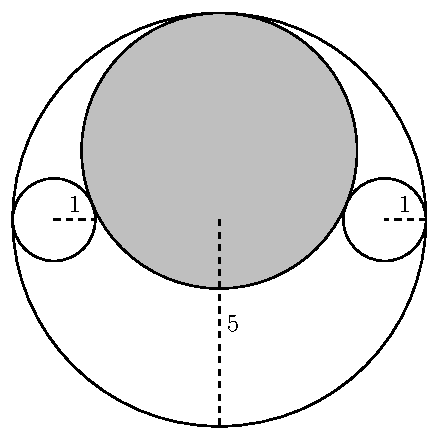
\includegraphics[height=10cm,page=1]{sprint-25-figure}
\end{center}

\nopagebreak

\begin{minipage}[b]{\linewidth}
\fbox{\phantom{ANSWER}}\\
\mbox{---------------}\\
\fbox{\phantom{ANSWER}}
\end{minipage}

\begin{answer}
\begin{center}
\includegraphics[height=10cm,page=2]{sprint-25-figure}
\end{center}
Consider the right triangle connecting the centers of one small circle, of the medium (shaded) circle and of the large circle. Let $r$ denote the (unknown) radius of the medium circle. The hypotenuse of the triangle has length $1+r$, the sum of the radius of the medium circle, $r$, and of the radius of the small circle, $1$. The shorter (vertical) leg of the triangle has length equal to the difference between the radius of the large circle and the radius of the medium circle, $5-r$. The longer (horizontal) leg of the triangle has length equal to the difference between the radius of the large circle and one of the small circles, or $5-1=4$. The radius $r$ can be found by applying the Pythagoras theorem:
\begin{align*}
4^2 + (5-r)^2 & = (r + 1)^2 \\
16 + 25 - 10r + r^2 & = r^2 + 2r + 1 
\quad\Rightarrow\quad
r = \frac{40}{12} = \frac{10}{3}
\end{align*}
\begin{empheq}[box={\mathbox[colback=white]}]{equation*}
    \frac{10}{3}
\end{empheq}
\end{answer}
%%%%%%%%%%%%%%%%%%%%%%%%%%%%%%%%%%%%%%%%%%%%%%%%%%%%%%%%%%%%%%%%%%%%%%%%

\iftoggle{showAnswers}{\newpage}

%%%%%%%%%%%%%%%%%%%%%%%%%%%%%%%%%%%%%%%%%%%%%%%%%%%%%%%%%%%%%%%%%%%%%%%%
\subsection*{26.}
The greatest of three nonnegative integers is one more than twice the sum of the other two integers. The arithmetic mean of the three integers, rounded to the nearest integer, happens to equal the median of the set. What is the product of the three integers?

\nopagebreak

\fbox{\phantom{ANSWER}}

\begin{answer}
Let $a \leq b \leq c$. We have (we guess strict inequalities because of the reference to ``rounding'', but rounding is consistent with one binding inequality):
\begin{align*}
& c \,=\, 1 + 2 (a + b) \\
& b - 1 \quad<\quad \frac{a + b + c}{3} \quad<\quad b + 1
\end{align*}
Eliminating $(a+b)=(c-1)/2$ by substitution yields: 
\begin{alignat*}{4}
b - 1 
    \quad & <
    \quad & 
        \frac{1}{3}\left(\frac{c-1}{2} + c\right) 
    \quad & < 
    \quad & \quad 
        b + 1 \\
\frac{6(b-1)+1}{3}
    \quad & <
    \quad & 
        c \quad\quad\;
    \quad & <
    \quad & \quad 
        \frac{6(b+1)+1}{3} \\
2b-1-\frac{2}{3}
    \quad & <
    \quad & 
        c \quad\quad\;
    \quad & <
    \quad & \quad 
        2b+2+\frac{1}{3}
\end{alignat*}
Since $2b-1$ and $2b+2$ are integers, we can simplify the inequality as:
\begin{align*}
2b-1 \quad\leq\quad c \quad\leq\quad 2b+2
\end{align*}
This inequality implies that $c$ could be equal to $2b-1$, $2b$, $2b+1$, or $2b+2$. But from $c=1+2(a+b)$, we can narrow down the guess to either $c=2b+1$ or $c=2b+2$. The first case implies $a=0$, which is not ruled out by the condition that the integers be ``nonnegative''. However we clearly must have $b>0$. The simplest guess is then $a=0$ and $b=1$, which yields $c=3$ and the inequality becomes $2 \leq 3 \leq  4$, which holds. This guess satisfies the conditions of the problem and the product of the integers is therefore
\begin{align*}
abc = 0 \times 1 \times 3 = 0
\end{align*}
\begin{empheq}[box={\mathbox[colback=white]}]{equation*}
    0
\end{empheq}
\end{answer}
%%%%%%%%%%%%%%%%%%%%%%%%%%%%%%%%%%%%%%%%%%%%%%%%%%%%%%%%%%%%%%%%%%%%%%%%

\iftoggle{showAnswers}{\newpage}

%%%%%%%%%%%%%%%%%%%%%%%%%%%%%%%%%%%%%%%%%%%%%%%%%%%%%%%%%%%%%%%%%%%%%%%%
\subsection*{27.}
Suppose $p(x)$ is a polynomial such that $p(x) = p(1) + p(2) \cdot x + x^2$ for all numbers $x$. What is the value of $p(5)$?

\nopagebreak

\fbox{\phantom{ANSWER}}

\begin{answer}
Setting $x=1$ yields:
\begin{align*}
p(1) = p(1) + p(2) \cdot 1 + 1^2
  \quad\Rightarrow\quad
p(2) = -1
\end{align*}
Setting $x=2$ yields:
\begin{align*}
p(2) = p(1) + p(2) \cdot 2 + 2^2
  \quad\Rightarrow\quad
-1 = p(1) - 2 + 4
  \quad\Rightarrow\quad
p(1) = -3
\end{align*}
The polynomial is therefore:
\begin{align*}
p(x) = -3 - x + x^2
\end{align*}
Setting $x=5$ yields:
\begin{align*}
p(5) = -3 - 5 + 5^2 = 17
\end{align*}
\begin{empheq}[box={\mathbox[colback=white]}]{equation*}
    17
\end{empheq}
\end{answer}
%%%%%%%%%%%%%%%%%%%%%%%%%%%%%%%%%%%%%%%%%%%%%%%%%%%%%%%%%%%%%%%%%%%%%%%%

\iftoggle{showAnswers}{\newpage}

%%%%%%%%%%%%%%%%%%%%%%%%%%%%%%%%%%%%%%%%%%%%%%%%%%%%%%%%%%%%%%%%%%%%%%%%
\subsection*{28.}
Let $\floor*{n}$ be defined as the greatest integer less than or equal to $n$. What is the value of $n$ if $\floor*{n} \times n = 3$? Express your answer as a decimal to the nearest tenth. 

\nopagebreak

\fbox{\phantom{ANSWER}}

\begin{answer}
If $n$ were an integer, the condition would reduce to $\floor*{n} \times n = n^2$ and
\begin{align*}
 n^2 = 3 \quad\Rightarrow\quad n \approx \pm 1.7
\end{align*}
The contradiction confirms that $n$ cannot be an integer. Furthermore it is clear that 
\begin{align*}
 1.0 < |n| < 1.7
\end{align*}
Since $\floor*{+1.x}=1$ for all digits $x$, it follows that $n$ must be negative. Since $\floor*{-1.x}=-2$, we have 
\begin{align*}
 \floor*{n} \times n = -2n = 3 \quad\Rightarrow\quad n = -1.5
\end{align*}
\begin{empheq}[box={\mathbox[colback=white]}]{equation*}
    -1.5
\end{empheq}
\end{answer}
%%%%%%%%%%%%%%%%%%%%%%%%%%%%%%%%%%%%%%%%%%%%%%%%%%%%%%%%%%%%%%%%%%%%%%%%

\iftoggle{showAnswers}{\newpage}

%%%%%%%%%%%%%%%%%%%%%%%%%%%%%%%%%%%%%%%%%%%%%%%%%%%%%%%%%%%%%%%%%%%%%%%%
\subsection*{29.}
Square ABCD, shown here, has side length $6$ units. Points P and Q are located on sides AD and BC, respectively, with $\text{AP}=\text{BQ}=1$ unit. Triangles ACP and BDQ overlap in the square to form the shaded quadrilateral. What is the area of the shaded quadrilateral? Express your answer as a common fraction. 

\begin{center}
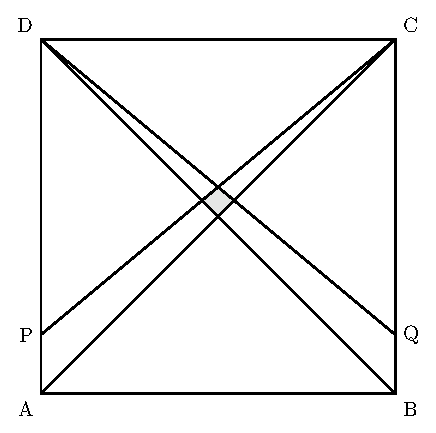
\includegraphics[height=10cm,page=1]{sprint-29-figure}
\end{center}

\nopagebreak

\begin{minipage}[b]{\linewidth}
\fbox{\phantom{ANSWER}}\\
\mbox{---------------}~~units$^2$\\
\fbox{\phantom{ANSWER}}
\end{minipage}


\begin{answer}
For clarity, add labels to the shaded quadrilateral: 
\begin{center}
\includegraphics[height=5cm,page=2]{sprint-29-figure}
\end{center}

In general, the area of a quadrilateral is equal to half the product of its diagonals. If we denote by $h$ the vertical diagonal, or `height', and by $w$ the horizontal diagonal, or `width', the area is equal to:
\begin{align*}
\frac{wh}{2}
\end{align*}
as can be seen from the figure (the area is half of the area of the four rectangles marked by dashed lines):
\begin{center}
\includegraphics[height=8cm,page=4]{sprint-29-figure}
\end{center}
Here the height is the distance OT, where O (`Origin') is the center of the square, and T is the intersection of CP and DQ. 

The height of the quadrilateral follows immediately from the ``Intercept theorem'' (known in France as Thales's theorem, but distinct from another theorem attributed to Thales that states that the triangle formed by the diameter of a circle and any other point on the circle has a right angle!). The Intercept theorem states that Given two parallel lines BD and CE and two non-parallel lines AC and AE, the following ratios hold:
\begin{align*}
\frac{\text{AC}}{\text{AB}} 
  = \frac{\text{AE}}{\text{AD}} 
  = \frac{\text{CE}}{\text{BD}} 
\end{align*} 
\begin{center}
\includegraphics[height=8cm,page=5]{sprint-29-figure}
\end{center}

Applying the Intercept Theorem to lines DB and DQ gives the height of the quadrilateral:
\begin{align*}
\frac{\text{DQ}}{\text{DT}} 
  = \frac{\text{DB}}{\text{DO}} 
  = \frac{\text{BQ}}{\text{OT}} 
\end{align*}
From $\text{DB}=2\text{DO}$ (the center of the square O cuts the diagonal DB in half) and $\text{BQ}=1$ (as stated in the question), it follows that the height of the quadrilateral is $\text{OT}=1/2$, or
\begin{align*}
h = \frac{1}{2}
\end{align*}
\begin{center}
\includegraphics[height=8cm,page=3]{sprint-29-figure}
\end{center}
Next, we calculate the width of the quadrilateral $w$. A simple method shown by Prof. Po Shen Loh is to consider the coordinate system centered at A and formed by an $x$-axis along AB and a $y$-axis along AD. In this system, the $x$-coordinate of the intersection of AC with DQ (point S) can be used to calculate distance RS (i.e. the width $w$). Namely, subtract the $x$-coordinate of O from the $x$-coordinate of S to get half the distance RS (i.e. $w/2$). 

In the coordinate system (AB, AD), the equations of AC and DQ are:
\begin{align*}
  \begin{cases}
  y = x \\
  y = 6 - \dfrac{5}{6}x
  \end{cases}
\end{align*}
The first equation is obvious, since AC is the diagonal of the square. The second equation holds because the $y$-intercept (distance AD) is $6$ and line DQ falls by $5$ units for every rightward displacement of $6$ units: equivalently, point Q is at coordinate $(6,1/6)$. 
Solving for the $x$-coordinate at the intersection of these two equations yields:
\begin{align*}
x = 6 - \frac{5}{6}x 
\quad\Rightarrow\quad 
x = \frac{36}{11}
\end{align*}
Since the $x$-coordinate of O is $3$, we get
\begin{align*}
\frac{w}{2} = \frac{36}{11} - 3 = \frac{3}{11}
\end{align*}
and the area is therefore 
\begin{align*}
h \times \frac{w}{2} = \frac{1}{2} \times \frac{3}{11} = \frac{3}{22}
\end{align*}
\begin{empheq}[box={\mathbox[colback=white]}]{equation*}
    \frac{3}{22}~\text{units}^2
\end{empheq}
\end{answer}
%%%%%%%%%%%%%%%%%%%%%%%%%%%%%%%%%%%%%%%%%%%%%%%%%%%%%%%%%%%%%%%%%%%%%%%%

\iftoggle{showAnswers}{\newpage}

%%%%%%%%%%%%%%%%%%%%%%%%%%%%%%%%%%%%%%%%%%%%%%%%%%%%%%%%%%%%%%%%%%%%%%%%
\subsection*{30.}
How many ordered triples of positive integers $(a,b,c)$ have $GCF(a,b,c)=2020$ and $LCM(a,b,c)=2020^2$?

\nopagebreak

\fbox{\phantom{ANSWER}}~ordered triples

\begin{answer}
As this is the last question of the Sprint round, we expect it to be quite difficult. Typical of competitions held in 2020-2021, the number $2020$ shows up. Its factors are easy to find if you know that $101$ is a prime number. But be prepared for $2021 = 43 \times 47$, which is not so obvious.
\begin{align*}
2020 = 2^2 \times 5 \times 101
\end{align*}
The problem's conditions may be written: 
\begin{align*}
GCF(a,b,c) & = 2^2 \cdot 5 \cdot 101 \\
LCM(a,b,c) & = 2^4 \cdot 5^2 \cdot 101^2
\end{align*}
The $GCF$ implies that $a$, $b$, $c$ are all divisible by $2$, $5$, $101$. The $LCM$ implies that they do not have any other prime factor. Thus, we have
\begin{align*}
a = 2^{\square} \times 5^{\square} \times 101^{\square} \\
b = 2^{\square} \times 5^{\square} \times 101^{\square} \\
c = 2^{\square} \times 5^{\square} \times 101^{\square} 
\end{align*}
for some integer powers to be determined. How many possibilities are there for these exponents? 

First consider the powers of $2$. 
Since $GCF\propto2^2$, the smallest power is $2^2$. 
Since $LCM\propto2^4$, the largest power is $2^4$. 
This gives three choices for assigning powers of $2$ to $(a,b,c)$:
\begin{align*}
(2^2, 2^2, 2^4) \quad\text{or}\quad 
(2^2, 2^4, 2^4) \quad\text{or}\quad 
(2^2, 2^3, 2^4)
\end{align*}
How many ways are there to assign the powers of $2$ to $(a,b,c)$?
There are $3$ ways to assign $(2^2,2^2,2^4)$. Likewise, there are $3$ ways to assign $(2^2,2^4,2^4)$. However, there are $6$ ways to assign $(2^2,2^3,2^4)$. Thus, there are $3+3+6=12$ ways to assign the powers of $2$. 

Now turn to the powers of $5$. 
How many ways are there to assign the powers of $5$ to $(a,b,c)$? 
They each have to be $5^1$ or $5^2$, so the powers of $5$ can be $(5^1,5^1,5^2)$ or $(5^1,5^2,5^2)$. There are $3$ ways to assign $(5^1,5^1,5^2)$ (to see this, choose whichever of the exponents is different from the other two). Thus, there are $3+3=6$ ways to assign $(5^1,5^1,5^2)$. 
Now turn to the powers of $101$. Just as for the powers of $5$, there are $6$ ways to assign the powers of $101$. 

Now consider all possible combinations. The total number of ways is obtained by multiplying the three cases, since the choice of the exponents for each prime are independent of each other:  
\begin{align*}
12 \times 6 \times 6 = 432
\end{align*}
ordered triples $(a,b,c)$.
\begin{empheq}[box={\mathbox[colback=white]}]{equation*}
    432 ~\text{ordered triples}
\end{empheq}
\end{answer}
%%%%%%%%%%%%%%%%%%%%%%%%%%%%%%%%%%%%%%%%%%%%%%%%%%%%%%%%%%%%%%%%%%%%%%%%


\end{document}